\section{Spin $1$ and higher spin}
\label{sec:one}

\subsection{Covariant reduction}

For spin $j$ let $\cQ_j$ be the set of unit-trace Hermitian operators on $\mathbb{C}^d$ with nonnegative Husimi function, $\langle\bq|Z|\bq\rangle\ge0$ for all $\bq$. These are the operators that give nonnegative probabilities on coherent projectors; they are dual to the mixtures of coherent states, the classical spin states of Ref.~\cite{giraud2008}. For a unit vector $\psi$, $Z\in\cQ_j$ and $l=1,\dots,2j$ define
\begin{equation}
m_l(\psi,Z)=\frac{d}{2l+1}\,\Tr\big(\Pi_l[|\psi\rangle\langle\psi|]\;\Pi_l[Z]\big).
\label{eq:ml}
\end{equation}

\begin{proposition}
\label{prop:cov}
Let all multipole ratios of the kernel $w$ be nonzero. The polarimeter is classical if and only if
$(\eta_1(w),\dots,\eta_{2j}(w))$ lies in the convex hull of the points $(m_1,\dots,m_{2j})(\psi,Z)$, $\psi$ a unit vector, $Z\in\cQ_j$.
\end{proposition}

The proof (Appendix~\ref{app:cov}) applies Lemma~\ref{lem:simplex}, transfers the kernel from the effects to the operators $Z_\lambda$ by Eq.~\eqref{eq:lambda}, and averages over rotations. The converse direction yields explicit models: the ontic states are the rotated copies of finitely many pairs $(\psi,Z)$.

For spin $1$, with the parametrisation of Eq.~\eqref{eq:symbol}, $\cQ\equiv\cQ_1$ is the set of pairs $(\bp,A)$ with
\begin{equation}
\tfrac23+\bp\!\cdot\!\bq+\bq^{\T}A\,\bq\ \ge0\quad\text{for all unit }\bq ,
\label{eq:Q1}
\end{equation}
and
\begin{equation}
m_1=\tfrac12\,\bp_\psi\!\cdot\!\bp_Z,\qquad m_2=\tfrac35\,\Tr(A_\psi A_Z).
\label{eq:m12}
\end{equation}
Every pure spin-$1$ state is a rotation of $\psi_\alpha=\cos\alpha\,\bm{e}_x+i\sin\alpha\,\bm{e}_y$ in the Cartesian basis, $0\le\alpha\le\pi/4$, for which $\bp=(0,0,\sin2\alpha)$ and $A=\operatorname{diag}(\tfrac13-\cos^2\!\alpha,\tfrac13-\sin^2\!\alpha,\tfrac13)$; $\alpha=0$ is linear polarisation (helicity $0$ along $x$) and $\alpha=\pi/4$ the coherent state.

\subsection{One spin-$1$ particle}

\begin{theorem}
\label{thm:one}
Let $\eta_2(w)\ne0$. The spin-$1$ polarimeter with kernel $w$ is classical if and only if
\begin{equation}
\begin{aligned}
&(\eta_1,\eta_2)\in\cR=\conv\big(\mathcal{L}\cup\{(0,-\tfrac45)\}\big),\\
&\mathcal{L}=\big\{3\eta_1^2+25\,(\eta_2-\tfrac15)^2\le1\big\}.
\end{aligned}
\label{eq:R}
\end{equation}
The support function of $\cR$ is
\begin{equation}
h_{\cR}(a,b)=\max\Big\{\tfrac b5+\sqrt{\tfrac{b^2}{25}+\tfrac{a^2}{3}},\ -\tfrac45b\Big\}.
\label{eq:hR}
\end{equation}
\end{theorem}

The boundary of $\cR$ consists of the arc of the ellipse above the points $(\pm\tfrac{2\sqrt2}{5},\tfrac{4}{25})$ and of the two segments from these points to the apex $(0,-\tfrac45)$ (Fig.~\ref{fig:regions}a). The ellipse is traced by a coherent $\psi$ together with the operators $Z_\tau$ for which the left-hand side of Eq.~\eqref{eq:Q1} is the square $(\sqrt{(2-\tau)/3}+\sqrt{\tau}\,q_z)^2$, $0\le\tau\le2$; they give $(m_1,m_2)=(\sqrt{\tau(2-\tau)/3},\tau/5)$; $\tau=\tfrac12$ is the coherent state itself, $(\tfrac12,\tfrac1{10})$, and $\tau=2$ gives the top $(0,\tfrac25)$, also obtained from $\psi=\bm{e}_x$, $Z=|\bm{e}_x\rangle\langle\bm{e}_x|$. The apex is $\psi=\bm{e}_x$, $Z=\openone-2|\bm{e}_x\rangle\langle\bm{e}_x|$, an operator that is not positive but has the nonnegative Husimi function $q_x^2$. The largest vector analysing power in $\cR$ is $|\eta_1|=1/\sqrt3$, at $\eta_2=\tfrac15$, i.e.\ $w=(0.655,0.267,0.078)$. The proof is in Appendix~\ref{app:spin1}; finite models at the extreme points are listed in Appendix~\ref{app:finite}.

\begin{figure*}[t]
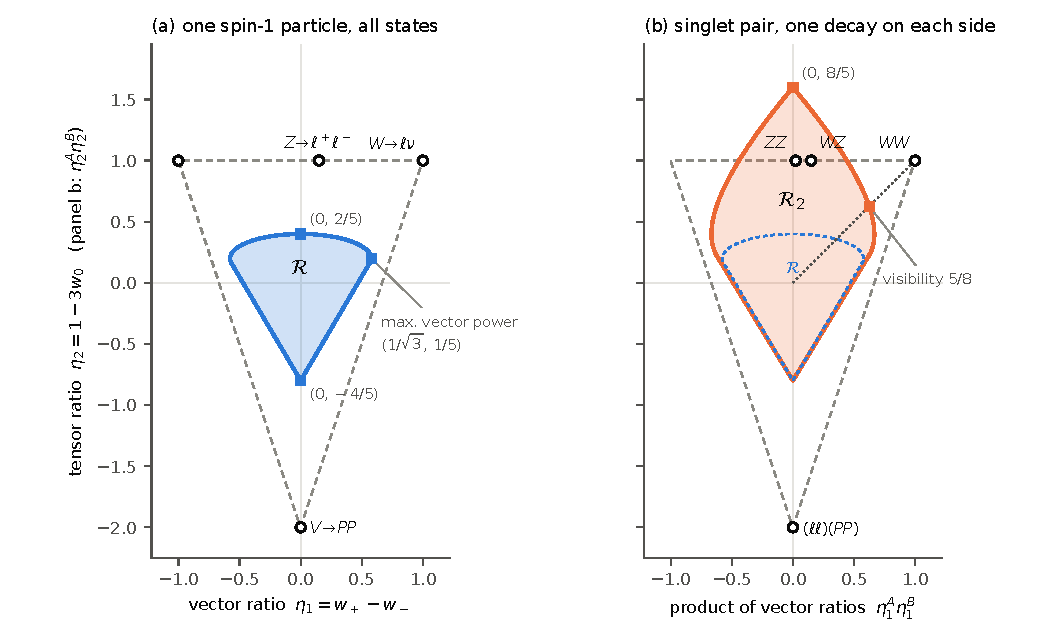
\includegraphics[width=0.78\textwidth]{fig_regions}
\caption{(a) Region $\cR$ of classical spin-$1$ polarimeters in the plane of the vector and tensor ratios (Theorem~\ref{thm:one}). The dashed triangle is the set of all kernels, $w\ge0$; its vertices are the helicity-pure decays. (b) Region $\cR_2$ for a spin-singlet pair with one decay on each side, in the plane of the products of the ratios (Theorem~\ref{thm:onepair}); the dotted line is the isotropic family for two $W\to\ell\nu$ decays, which leaves $\cR_2$ at visibility $5/8$. The dashed outline in (b) repeats $\cR$.}
\label{fig:regions}
\end{figure*}

The set of all kernels is the triangle with vertices $(\eta_1,\eta_2)=(1,1)$, $(-1,1)$, $(0,-2)$, which correspond to $w=(1,0,0)$, $(0,0,1)$, $(0,1,0)$. All three, and the whole edge $\eta_2=1$, lie outside $\cR$: no decay that fixes the helicity along the recorded direction is a classical polarimeter.

\begin{corollary}[Parity-symmetric kernels]
\label{cor:parity}
If $w_+=w_-$, the polarimeter is classical if and only if $\tfrac15\le w_0\le\tfrac35$. For a decay whose direction is distributed as $1+\alpha\cos^2\theta$ about the spin axis of a parent with helicity $\pm1$ this is $-\tfrac12\le\alpha\le\tfrac13$; for a decay into a fermion pair through a vector current, $\alpha=(1-4x)/(1+4x)$ with $x=m_f^2/M^2$, it is $x\ge\tfrac18$.
\end{corollary}

\begin{proof}
$\eta_1=0$ and $-\tfrac45\le\eta_2\le\tfrac25$; $w_0=(1-\alpha)/(3+\alpha)$.
\end{proof}

\begin{remark}[Degenerate kernels]
\label{rem:deg}
For $\eta_1=0\ne\eta_2$ the effects do not separate states that differ only in $\bp$; the criterion of Theorem~\ref{thm:one} remains valid, under both readings, because the end points of the segment $\cR\cap\{\eta_1=0\}$ are realised with $\bp_\psi=\bp_Z=0$ (Appendix~\ref{app:spin1}). For $\eta_2=0$ exactly the situation changes: the data depend on the state through $\bp$ only, $p(\bq)=\frac{1}{4\pi}(1+\tfrac32\eta_1\,\bp\!\cdot\!\bq)$ with $|\bp|\le1$, and Theorem~\ref{thm:half} gives the criterion $|\eta_1|\le\tfrac29$ under reading I; under reading II it is $|\eta_1|\le\tfrac13$. Both are smaller than the limit $\sqrt2/3$ of $\cR$ as $\eta_2\to0$. The set of classical kernels is thus not closed at $\eta_2=0$: for $\eta_2\ne0$, however small, a response function may contain a quadrupole term $\bq^{\T}\tilde A\bq$ of order one, because the effects contain a small quadrupole component to which it is attached linearly; at $\eta_2=0$ no effect carries such a component. A noncontextuality test near $\eta_2=0$ is correspondingly sensitive to the precision with which the equivalences are established \cite{mazurek2016,pusey2018}.
\end{remark}

\subsection{Spin-singlet pair of spin-$1$ particles}

Theorem~\ref{thm:pair}(b) has a counterpart for arbitrary spins. Let particles $A$ and $B$ of spins $j_A$, $j_B$ in a state $\rho$ decay through polarimeters with kernels $w^A$, $w^B$, and let $\cF_{B\to A}$ be the fragment of the states of $A$ steered by outcome sets of $B$, $\omega(\bq_B)=\Tr_B[\rho\,(\openone\otimes E_{w^B}(\bq_B))]$ and their mixtures, with the effects of $A$.

\begin{proposition}
\label{prop:pairpoly}
(i) If $\cF_{B\to A}$ has a noncontextual model, under either reading, then
\begin{equation}
p(\bq_A,\bq_B)=\sum_\lambda r_\lambda(\bq_A)\,s_\lambda(\bq_B)
\label{eq:pairpoly}
\end{equation}
with finitely many nonnegative polynomials $r_\lambda$, $s_\lambda$ on the sphere of degree at most $2j_A$ and $2j_B$.
(ii) If all multipole ratios of both kernels are nonzero and the map $X\mapsto\Tr_B[\rho\,(\openone\otimes X)]$ from Hermitian operators of $B$ to those of $A$ is invertible, the converse holds.
\end{proposition}

\begin{proof}
(i) In a noncontextual model $e(\omega)=\sum_\lambda e(Z_\lambda)g_\lambda(\omega)$ for all effects and states of the fragment. Put $r_\lambda(\bq_A)=\Tr[Z_\lambda E_{w^A}(\bq_A)]$ and $s_\lambda(\bq_B)=g_\lambda(\omega(\bq_B))$. Both are nonnegative, and both are linear functionals of operators whose matrix elements are polynomials of degree $2j$ in the direction. (ii) Under the hypotheses each polynomial of degree $2j_A$ is $\Tr[ZE_{w^A}(\bq_A)]$ for a unique Hermitian $Z$, each polynomial of degree $2j_B$ is $g(\omega(\bq_B))$ for a unique functional $g$, and the states and effects of the fragment span the full operator space, so that Eq.~\eqref{eq:pairpoly} is Eq.~\eqref{eq:simplex}.
\end{proof}

Equation~\eqref{eq:pairpoly} is a local hidden-variable model whose response functions are polynomials of bounded degree; the recorded-outcome model of Remark~\ref{rem:lhv} uses delta functions instead. For spin $1/2$ nonnegative polynomials of degree one are the elements of the Bloch cone and Eq.~\eqref{eq:pairpoly} is Eq.~\eqref{eq:localnc}; Theorem~\ref{thm:pair} shows that the invertibility hypothesis of (ii) is not needed there.

Let $|\Psi_0\rangle=\tfrac{1}{\sqrt3}\sum_m(-1)^{1-m}|m\rangle|{-m}\rangle$ be the state of total spin zero of two spin-$1$ particles and $\rho_v=v|\Psi_0\rangle\langle\Psi_0|+(1-v)\openone/9$ the isotropic family; $\rho_v$ is entangled if and only if $v>\tfrac14$ \cite{horodecki1999}. Each particle decays through a polarimeter, with kernels $w^A$ and $w^B$.

\begin{theorem}
\label{thm:onepair}
Let $\eta_2^A\eta_2^B\ne0$. The decay data of $\rho_v$ have a noncontextual model if and only if
\begin{equation}
\big(v\,\eta_1^A\eta_1^B,\ v\,\eta_2^A\eta_2^B\big)\in\cR_2=\conv\big(\Gamma\cup\Gamma^-\cup\{(0,-\tfrac45)\}\big),
\label{eq:R2}
\end{equation}
where $\Gamma=\{(\tfrac23s(2-s),\tfrac25s^2):0\le s\le2\}$ and $\Gamma^-$ is its mirror image under $\eta_1\to-\eta_1$. The support function is
\begin{equation}
h_{\cR_2}(a,b)=\max\Big\{\max_{0\le s\le2}\big[\tfrac23|a|\,s(2-s)+\tfrac25b\,s^2\big],\ -\tfrac45b\Big\}.
\label{eq:hR2}
\end{equation}
\end{theorem}

The boundary of $\cR_2$ consists of the arcs $\sqrt3-1\le s\le2$ of $\Gamma$ and $\Gamma^-$, which meet at $(0,\tfrac85)$, and of the segments from $\Gamma(\sqrt3-1)$ and its mirror image to $(0,-\tfrac45)$ (Fig.~\ref{fig:regions}b). $\cR_2$ is larger than $\cR$ because the states steered through a decay are images of the coherent cone only, not all states; the functionals $g_\lambda$ then need to be nonnegative on fewer states, and both factors of the model range over $\cQ$ (Appendix~\ref{app:spin1}).

\begin{table}[t]
\caption{Critical visibility $v_c$ of the isotropic spin-$1$ pair state for pairs of decays: the data are contextual if and only if $v>v_c$ (the state is entangled if and only if $v>1/4$). $V\to PP$ is a decay of a vector particle into two pseudoscalars, $V\to\ell\ell$ into a massless lepton pair through a vector current; $A_\ell$ is the leptonic asymmetry parameter of the $Z$.}
\label{tab:pairs}
\begin{ruledtabular}
\begin{tabular}{lcc}
Decays & $(\eta_1^A\eta_1^B,\ \eta_2^A\eta_2^B)$ & $v_c$\\
\hline
$W\to\ell\nu$, $W\to\ell\nu$ & $(\pm1,\ 1)$ & $5/8$\\
$W\to\ell\nu$, $Z\to\ell\ell$ & $(\pm A_\ell,\ 1)$ & none\\
$Z\to\ell\ell$, $Z\to\ell\ell$ & $(A_\ell^2,\ 1)$ & none\\
$V\to\ell\ell$, $V\to\ell\ell$ & $(0,\ 1)$ & none\\
$V\to PP$, $V\to PP$ & $(0,\ 4)$ & $2/5$\\
$V\to PP$, $V\to\ell\ell$ or $W\to\ell\nu$ & $(0,\ -2)$ & $2/5$\\
\end{tabular}
\end{ruledtabular}
\end{table}

\begin{corollary}
\label{cor:vis}
The critical visibilities of Table~\ref{tab:pairs} hold. In particular two ideal $W\to\ell\nu$ decays on a singlet give contextual data if and only if $v>5/8$, and with a $Z\to\ell\ell$ decay on at least one side the data are noncontextual for every $v$.
\end{corollary}

\begin{proof}
The ray $v(1,1)$ meets $\Gamma$ at $s=\tfrac54$, $v=\tfrac58$, on the curved part of the boundary. On the axis $\eta_1=0$, $\cR_2$ is the interval $[-\tfrac45,\tfrac85]$. At $\eta_2^A\eta_2^B=1$ the boundary is at $\eta_1^A\eta_1^B=\tfrac23\sqrt{10}-\tfrac53\approx0.44$, which exceeds $A_\ell=\Ae\pm\AeErr$ \cite{pdg2026}.
\end{proof}

\subsection{Spin $j$}

Let $\xi_{2j}$ denote the largest node of the Gauss--Legendre rule with $j+1$ nodes (the largest zero of the Legendre polynomial $P_{j+1}$) if $j$ is an integer, and the largest node of the Gauss--Radau rule with $j+\tfrac32$ nodes, one of them fixed at $-1$ (the largest zero of $(P_n+P_{n+1})/(1+t)$ with $n=j+\tfrac12$), if $j$ is a half-integer \cite{gautschi2004}.

\begin{theorem}
\label{thm:spinj}
(a) Every classical polarimeter of spin $j$ has vector analysing power $|\kappa_1|\le\xi_{2j}$, under either reading and for any kernel.
(b) The bound is the supremum over classical polarimeters. It is attained by the kernel $D^\star=\frac{d}{4\pi}\int d\bq\,Q^\star(\bq)\,|\bq\rangle\langle\bq|$, where $Q^\star$ is the nonnegative polynomial of degree $2j$ in $q_z$ that vanishes at all nodes except the largest, normalised to $\Tr D^\star=1$, provided all multipole ratios of $D^\star$ are nonzero; this holds for $j\le4$.
(c) For two particles of spins $j_A$, $j_B$ in any state and with any kernels, noncontextual decay data satisfy
\begin{equation}
\big\|\langle\bq_A\bq_B^{\T}\rangle\big\|_1\le\xi_{2j_A}\,\xi_{2j_B},
\label{eq:dipole}
\end{equation}
where $\langle\bq_A\bq_B^{\T}\rangle$ is the $3\times3$ matrix of the moments $\langle q_{A,i}q_{B,k}\rangle$ and $\|\cdot\|_1$ the trace norm. In particular $|\langle\bq_A\!\cdot\!\bq_B\rangle|\le\xi_{2j_A}\xi_{2j_B}$.
\end{theorem}

\begin{proof}[Proof of (a)]
In a noncontextual model $E_w(\bq)=\sum_\lambda G_\lambda\,r_\lambda(\bq)$ with $G_\lambda\ge0$, $\sum_\lambda G_\lambda=\openone$, and $r_\lambda(\bq)=\Tr[Z_\lambda E_w(\bq)]$ a nonnegative polynomial of degree at most $2j$ with $\int d\bq\,r_\lambda=1$ (Remark~\ref{rem:lhv}, Eq.~\eqref{eq:lambda}). Multiplying by $\bq$, integrating and using Eq.~\eqref{eq:firstmoment}, $\kappa_1\bJ/(j+1)=\sum_\lambda G_\lambda\,\bx_\lambda$ with $\bx_\lambda=\int d\bq\,\bq\,r_\lambda(\bq)$. Taking the trace with $\bJ$ and using $\Tr(\bJ\!\cdot\!\bJ)=j(j+1)d$ and $|\bx\!\cdot\!\Tr(G\bJ)|\le j|\bx|\Tr G$ for $G\ge0$ gives $|\kappa_1|\le\max_\lambda|\bx_\lambda|$. Averaging $r_\lambda$ over rotations about $\bx_\lambda$ gives a nonnegative polynomial $f$ of degree at most $2j$ in $t=\bq\!\cdot\!\hat{\bx}_\lambda$ with $\int_{-1}^1f\,dt=1$ and $|\bx_\lambda|=\int_{-1}^1t\,f(t)\,dt$. The quadrature rule named above has positive weights $\omega_k$ and is exact for polynomials of degree $2j+1$, hence for $f$ and $tf$: $\int tf=\sum_k\omega_kt_kf(t_k)\le\xi_{2j}\sum_k\omega_kf(t_k)=\xi_{2j}$.
\end{proof}

\begin{proof}[Proof of (c)]
By Proposition~\ref{prop:pairpoly}(i), $p=\sum_\lambda\pi_\lambda\hat r_\lambda(\bq_A)\hat s_\lambda(\bq_B)$ with weights $\pi_\lambda\ge0$ summing to one and normalised nonnegative polynomials of degree at most $2j_A$, $2j_B$. Their first moments $\bx_\lambda$, $\bm{y}_\lambda$ obey $|\bx_\lambda|\le\xi_{2j_A}$, $|\bm{y}_\lambda|\le\xi_{2j_B}$ by the argument of (a), and $\langle\bq_A\bq_B^{\T}\rangle=\sum_\lambda\pi_\lambda\bx_\lambda\bm{y}_\lambda^{\T}$ has trace norm at most $\sum_\lambda\pi_\lambda|\bx_\lambda||\bm{y}_\lambda|$.
\end{proof}

Part (b) is proved in Appendix~\ref{app:spinj}. Table~\ref{tab:gj} lists the values; $\xi_1=\tfrac13$ and $\xi_2=1/\sqrt3$ reproduce Theorems~\ref{thm:half} and \ref{thm:one}, $\xi_3=(1+\sqrt6)/5$, $\xi_4=\sqrt{3/5}$, and $\xi_{2j}\to1$ for $j\to\infty$: for large spin a classical polarimeter can be almost sharp in its vector part. Part (c) is a test on nine first moments of the data that needs neither the state nor the kernels. For two spin-$1/2$ particles $\langle\bq_A\bq_B^{\T}\rangle=c/9$ and Eq.~\eqref{eq:dipole} is $\|c\|_1\le1$, which is therefore necessary for polarised pairs as well and contains Corollary~\ref{cor:D}. For the spin-$1$ pair state $\rho_v$, $\langle\bq_A\bq_B^{\T}\rangle=-\tfrac16v\,\eta_1^A\eta_1^B\,\openone_3$, and Eq.~\eqref{eq:dipole} reads $v|\eta_1^A\eta_1^B|\le\tfrac23$, the largest abscissa of $\cR_2$: the inequality is tight for $j=\tfrac12$ and $j=1$ in this sense, although it is weaker than Theorems~\ref{thm:pair} and \ref{thm:onepair} away from that direction (it gives $v\le\tfrac23$ instead of $\tfrac58$ for two $W\to\ell\nu$ decays).

\begin{table}[t]
\caption{Largest vector analysing power $\xi_{2j}$ of a classical spin-$j$ polarimeter (Theorem~\ref{thm:spinj}) and the value of the linear programme that maximises the first moment over operators with nonnegative Husimi function (Appendix~\ref{app:numerics}).}
\label{tab:gj}
\begin{ruledtabular}
\begin{tabular}{llll}
$j$ & Quadrature rule & $\xi_{2j}$ & LP value \\
\hline
$1/2$ & Gauss--Radau, 2 nodes & 0.333333 & 0.333333 \\
$1$ & Gauss--Legendre, 2 nodes & 0.577350 & 0.577350 \\
$3/2$ & Gauss--Radau, 3 nodes & 0.689898 & 0.689898 \\
$2$ & Gauss--Legendre, 3 nodes & 0.774597 & 0.774597 \\
$5/2$ & Gauss--Radau, 4 nodes & 0.822824 & 0.822824 \\
$3$ & Gauss--Legendre, 4 nodes & 0.861136 & 0.861137 \\
$7/2$ & Gauss--Radau, 5 nodes & 0.885792 & 0.885792 \\
$4$ & Gauss--Legendre, 5 nodes & 0.906180 & 0.906180 \\
\end{tabular}
\end{ruledtabular}

\end{table}
